\begin{figure}
\centering	
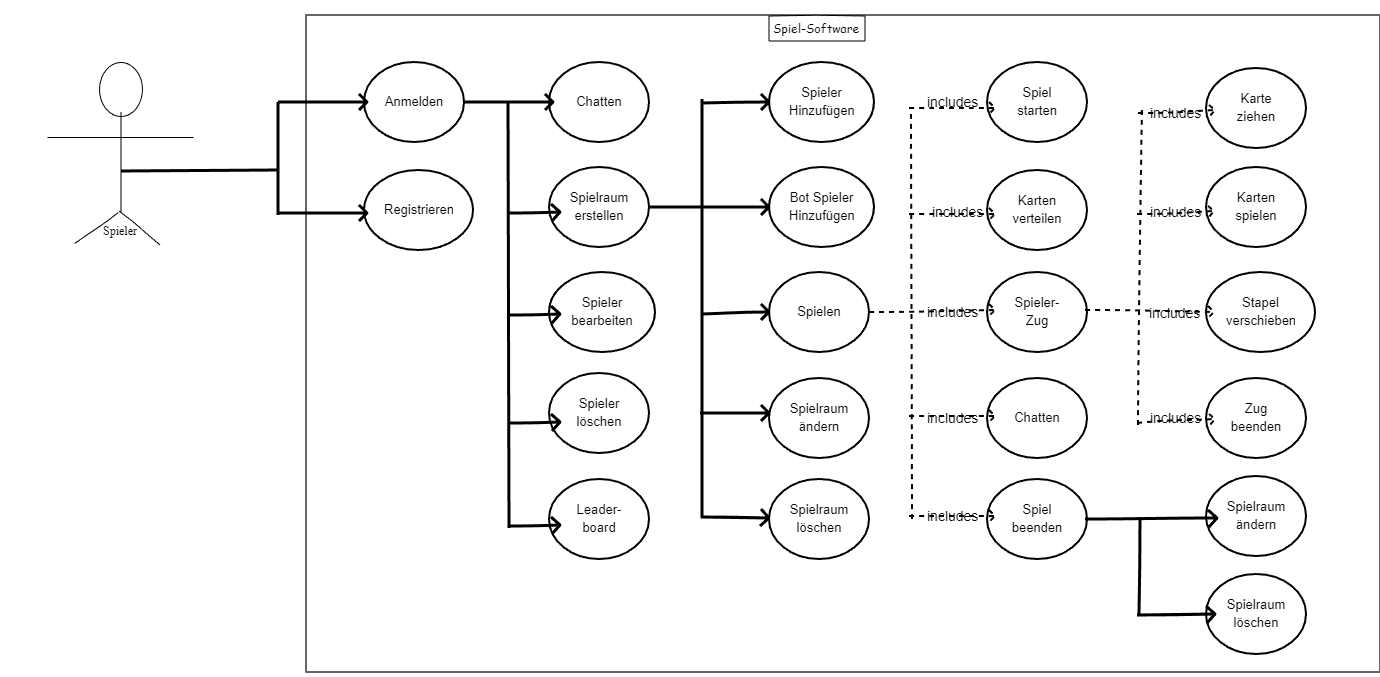
\includegraphics[width=1.1\textwidth]{img/ucd.png}
\label{fig:sys}
\caption{Beispiel für ein Systemgrenzendiagramm (Use Case Diagramm), das vor Abgabe anzupassen ist.}
\end{figure}

\section{Systemgrenze (Use Case Diagramm)}

Die Systemgrenze wird in der Abbildung~\ref{fig:sys} dargestellt\footnote{Weitere Erklärungen und Spezifizierungen, die sich auf Abgrenzungen der Verantwortlichkeiten vom System und weiteren Akteuren/Systemen beziehen, können hier spezifiziert werden.}. 


\section{Beschreibungen der Anwendungsfälle}

%Hinweis: Alle Systemfunktionen sind mit Anwendungsfällen zu decken! (Und dieser Hinweis ist zu löschen, wie auch der Beispielfall).

\newcounter{uc}\setcounter{uc}{10}

\begin{description}[leftmargin=5em, style=sameline]
	
	\begin{lhp}{uc}{UC}{uc:anmeld}
		\item [Name:] Spieler anmelden.
		\item [Ziel:] Spieler meldet sich im System an.
		\item [Akteure:] Spieler.
		\item [Vorbedingungen] Spieler ist im Vorraum.
		\item [Eingabedaten:] Zugriffsdaten~\ref{daten:benutzername}~\ref{daten:passwort}.
		\item [Beschreibung:] Spieler meldet sich an.							
		\item [Ausnahmen:] \hfill
			\begin{itemize} 
				\item[] \textit{Passwort oder Benutzername ist falsch:} Das System zeigt eine Fehlermeldung an, anstatt des Schrittes 2.
				
			\end{itemize}
		\item [Ergebnisse und Outputdaten:] Spieler ist in der Lobby und sieht die Bestenliste.	
		\item [Systemfunktionen:] \ref{funk:zugriff}.
	\end{lhp}
	
	\begin{lhp}{uc}{UC}{uc:registrieren}
		\item [Name:] Spieler registrieren
		\item [Ziel:] Spieler registriert einen Account im System.
		\item [Akteure:] Spieler.
		\item [Vorbedingungen:] Spieler ist im Vorraum.
		\item [Eingabedaten:] Zugriffsdaten~\ref{daten:benutzername}, Passwort~\ref{daten:passwort}.
		\item [Beschreibung:] Spieler registriert sich.
		\item [Ausnahmen:] \hfill
			\begin{itemize} 
				\item[] \textit{Benutzername ist schon vergeben:} Das System zeigt eine Fehlermeldung an, anstatt des Schrittes 2.
				
				\item[] \textit{Passwort entspricht nicht den Vorgaben:} Das System zeigt eine Fehlermeldung an, anstatt des Schrittes 2.
				
			\end{itemize}
		\item [Ergebnisse und Outputdaten:] Neuer Account wurde angelegt. Spieler ist im Vorraum und kann sich nun anmelden.
		\item [Systemfunktionen] \ref{funk:zugriff}.
	\end{lhp}
	
	\begin{lhp}{uc}{UC}{uc:chatten}
		\item [Name:] Chatten
		\item [Ziel:] Spieler benutzt den Chat.
		\item [Akteure:] Spieler.
		\item [Vorbedingungen:] Spieler ist in der Lobby oder einer Spielrunde.
		\item [Eingabedaten:] Chatverlauf~\ref{daten:chatverlauf}, Chat-Eingabe~\ref{daten:chat-eingabe}.
		\item [Beschreibung:] Ein Spieler schreibt eine Nachricht.
		\item [Ausnahmen:] \hfill
			\begin{itemize} 
				\item[] \textit{Die Chatnachricht enhält laut AGBs nicht erlaubte Teilworte:} Das System zeigt eine Warnmeldung an, die Nachricht wird nicht in den Chatverlauf aufgenommen.
				
			\end{itemize}
		\item [Ergebnisse und Outputdaten:] Die Nachricht ist im Chatverlauf sichtbar.
		\item [Systemfunktionen] \ref{funk:chat}.
	\end{lhp}
	
	\begin{lhp}{uc}{UC}{uc:erstellen}
		\item [Name:] Spielraum erstellen.
		\item [Ziel:] Spieler erstellt Spielraum.
		\item [Akteure:] Spieler.
		\item [Vorbedingungen] Spieler ist in der Lobby.
		\item [Eingabedaten:] Spielraumdaten~\ref{daten:spielraumname}\ref{daten:spielraumpasswort}.
		\item [Beschreibung:] Spieler erstellt einen neuen Spielraum.
		\item [Ausnahmen:] \hfill
			\begin{itemize} 
				\item[] \textit{Spielname ist schon vergeben:} Das System zeigt eine Fehlermeldung an, anstatt des Schrittes 2.
				
				\item[] \textit{Passwort entspricht nicht den Vorgaben:} Das System zeigt eine Fehlermeldung an, anstatt des Schrittes 2.
				
			\end{itemize}
		\item [Ergebnisse und Outputdaten:] Spieler ist im neu erstellten Spielraum.	
		\item [Systemfunktionen:] \ref{funk:zugriff}.
	\end{lhp}
	
	\begin{lhp}{uc}{UC}{uc:bearbeiten}
		\item [Name:] Spieler bearbeiten
		\item [Ziel:] Spieler bearbeitet seine Daten.
		\item [Akteure:] Spieler.
		\item [Vorbedingungen:] Spieler ist in der Lobby.
		\item [Eingabedaten:] Zugriffsdaten~\ref{daten:benutzername}~\ref{daten:passwort}.
		\item [Beschreibung:] Spieler bearbeitet seine Accountdaten.
		\item [Ausnahmen:] \hfill
			\begin{itemize} 
			    \item[] \textit{Passwort ist falsch:} Das System zeigt eine Fehlermeldung an, anstatt des Schrittes 2.
			    
				\item[] \textit{Neuer Benutzername ist schon vergeben:} Das System zeigt eine Fehlermeldung an, anstatt des Schrittes 2.
				
				\item[] \textit{Neues Passwort entspricht nicht den Vorgaben:} Das System zeigt eine Fehlermeldung an, anstatt des Schrittes 2.
				
			\end{itemize}
		\item [Ergebnisse und Outputdaten:] Spieler ist in der Lobby. Die Daten des Acounts wurden bearbeitet.
		\item [Systemfunktionen] \ref{funk:zugriff}.
	\end{lhp}
	
	\begin{lhp}{uc}{UC}{uc:löschen}
		\item [Name:] Spieler löschen.
		\item [Ziel:] Spieler entfernt seine Daten aus dem System.
		\item [Akteure:] Spieler.
		\item [Vorbedingungen] Spieler ist in der Lobby.
		\item [Eingabedaten:] Passwort~\ref{daten:passwort}.
		\item [Beschreibung:] Spieler löscht das eigene Konto komplett.
		\item [Ausnahmen:] \hfill
			\begin{itemize} 
				\item[] \textit{Passwort ist falsch:} Das System zeigt eine Fehlermeldung an, anstatt des Schrittes 2.
				\item[] \textit{Keine Löschung erwünscht:} Anstatt des Schrittes 4, schließt das System den Dialog.
				
			\end{itemize}
		\item [Ergebnisse und Outputdaten:] Spieler ist im Vorraum, Spielerkonto wurde gelöscht.	
		\item [Systemfunktionen:] \ref{funk:zugriff}.
	\end{lhp}
	
	\begin{lhp}{uc}{UC}{uc:leaderboard}
		\item [Name:] Leaderboard.
		\item [Ziel:]Spieler sieht die Highscores aller Spieler.
		\item [Akteure:] Spieler.
		\item [Vorbedingungen] Spieler ist in der Lobby.
		\item [Eingabedaten:] Highscores~\ref{daten:highscores}.
		\item [Beschreibung:] Spieler lässt sich die Highscores aller Spieler anzeigen.
		\item [Ausnahmen:] \hfill
			\begin{itemize} 
				\item[] \textit{Keine Highscores vorhanden:} Das System zeigt eine Hinweismeldung an, anstatt des Schrittes 2.
				
			\end{itemize}
		\item [Ergebnisse und Outputdaten:] Spieler ist in der Lobby, sieht das Leaderboard.	
		\item [Systemfunktionen:] \ref{funk:bestenliste}.
	\end{lhp}
	
	\begin{lhp}{uc}{UC}{uc:Hinzufügen}
		\item [Name:] Spieler hinzufügen.
		\item [Ziel:] Einen Spieler zu einem Spielraum hinzufügen.
		\item [Akteure:] Spieler.
		\item [Vorbedingungen] Spieler ist Host eines Spielraums.
		\item [Eingabedaten:] Benutzername~\ref{daten:benutzername}.
		\item [Beschreibung:] Spieler lädt einen anderen Spieler in seinen Spielraum ein.
		\item [Ausnahmen:] \hfill
			\begin{itemize} 
				\item[] \textit{Spieler mit angegebenen Benutzername ist nicht verfügbar:} Das System zeigt eine Fehlermeldung an, anstatt des Schrittes 2.
				
			\end{itemize}
		\item [Ergebnisse und Outputdaten:] Spieler ist im Spielraum, der andere Spieler erhält eine Einladung.	
		\item [Systemfunktionen:] \ref{funk:spielraum}.
	\end{lhp}
	
	\begin{lhp}{uc}{UC}{uc:hinzufügen}
		\item [Name:] Bot-Spieler hinzufügen.
		\item [Ziel:] Einen Bot-Spieler zu einem Spielraum hinzufügen.
		\item [Akteure:] Spieler.
		\item [Vorbedingungen] Spieler ist Host eines Spielraums.
		\item [Eingabedaten:] Botname~\ref{daten:botname}.
		\item [Beschreibung:] Spieler fügt einen Bot-Spieler in seinen Spielraum hinzu.
		\item [Ausnahmen:] \hfill
			\begin{itemize} 
				\item[] \textit{Botname ist schon vergeben:} Das System zeigt eine Fehlermeldung an, anstatt des Schrittes 2.
				
			\end{itemize}
		\item [Ergebnisse und Outputdaten:] Spieler ist im Spielraum, der andere Spieler erhält eine Einladung.	
		\item [Systemfunktionen:] \ref{funk:spielraum}\ref{funk:bots}.
	\end{lhp}
	
	\begin{lhp}{uc}{UC}{uc:Spielen}
		\item [Name:] Spielen.
		\item [Ziel:] Eine Spielrunde beginnen.
		\item [Akteure:] Spieler, Bot-Spieler.
		\item [Vorbedingungen] Spieler sind in einem Spielraum.
		\item [Eingabedaten:] Karten~\ref{daten:karten}, Kartenstappel~\ref{daten:kartenstappel}, Handkarten~\ref{daten:handkarten} 
		\item [Beschreibung:] Host beginnt eine Spielrunde.
		\item [Ausnahmen:] \hfill
			\begin{itemize} 
				\item[] \textit{Nicht genügend Spieler vorhanden:} Das System zeigt eine Fehlermeldung an, anstatt des Schrittes 2.
				
			\end{itemize}
		\item [Ergebnisse und Outputdaten:] Es wird eine neue Spielrunde begonnen mit den Teilnehmern im Spielraum.	
		\item [Systemfunktionen:] \ref{funk:spielraum}\ref{funk:bots}\ref{funk:chat}.
	\end{lhp}
	
	\begin{lhp}{uc}{UC}{uc:Starten}
		\item [Name:] Spiel starten.
		\item [Ziel:] Spieler werden in eine Spielumgebung transferriert.
		\item [Akteure:] System der Spielraumverwaltung.
		\item [Vorbedingungen] Ein neues Spiel wurde begonnen.
		\item [Eingabedaten:] .
		\item [Beschreibung:] Spieler werden in eine neue Spielumgebung transferiert.
		\item [Ausnahmen:] .
		\item [Ergebnisse und Outputdaten:] Die teilnehmenden Spieler befinden sich in einer Spielumgebung.
		\item [Systemfunktionen:] \ref{funk:spielraum}.
	\end{lhp}
	
	\begin{lhp}{uc}{UC}{uc:Verteilen}
		\item [Name:] Karten verteilen.
		\item [Ziel:] Ausgangssituation einer neuen Spielrunde herstellen.
		\item [Akteure:] System der Spielraumverwaltung.
		\item [Vorbedingungen] Ein neues Spiel wurde begonnen.
		\item [Eingabedaten:] Karten~\ref{daten:karten}, Kartenstappel~\ref{daten:kartenstappel}, Handkarten~\ref{daten:handkarten} 
		\item [Beschreibung:] Kartenstappel werden erstellt und Handkarten ausgeteilt.
		\item [Ausnahmen:] .
		\item [Ergebnisse und Outputdaten:] Die Anfangskartenstappel wurden erstellt und jedem Spieler wurde die richtige Anzahl an Handkarten ausgeteilt.
		\item [Systemfunktionen:] \ref{funk:spielraum}.
	\end{lhp}
	
	\begin{lhp}{uc}{UC}{uc:Zug}
		\item [Name:] Spieler-Zug.
		\item [Ziel:] Ein Spieler führt einen Zug aus.
		\item [Akteure:] Spieler, Bot-Spieler.
		\item [Vorbedingungen] Spieler ist am Zug.
		\item [Eingabedaten:] Karten~\ref{daten:karten}, Kartenstappel~\ref{daten:kartenstappel}, Handkarten~\ref{daten:handkarten} 
		\item [Beschreibung:] Ein Spieler zieht eine Karte und führt seinen Zug nach den Spielregeln aus. Er wählt dabei aus den folgenden Optionen
		\item [Ausnahmen:] \hfill
			\begin{itemize} 
				\item[] \textit{Der Spieler führt für eine festgelegte Zeit keine Operation aus:} Der Zug des
				Spielers wird vom System beendet und der nächste Spieler ist am Zug.
			\end{itemize}
		\item [Ergebnisse und Outputdaten:] Ein Spieler hat seinen Zug ausgeführt und der nächste Spieler ist an der Reihe.
		\item [Systemfunktionen:] \ref{funk:spielraum}\ref{funk:bots}.
	\end{lhp}
	
	\begin{lhp}{uc}{UC}{uc:Spiel_beenden}
		\item [Name:] Spiel beenden.
		\item [Ziel:] Das Spiel wird beendet.
		\item [Akteure:] Spieler, Bot-Spieler, System der Spielraumverwaltung.
		\item [Vorbedingungen] Der Host beendet das Spiel oder ein Spieler hat keine Handkarten mehr.
		\item [Eingabedaten:] Karten~\ref{daten:karten}, Kartenstappel~\ref{daten:kartenstappel}, Handkarten~\ref{daten:handkarten}, Highscores~\ref{daten:highscores} 
		\item [Beschreibung:] Der Spielhost beendet die Spielrunde oder ein Spieler hat gewonnen, da er keine Karten mehr auf der Hand hat.
		\item [Ausnahmen:] \hfill
			\begin{itemize} 
				\item[] \textit{Alle Teilnehmer sind für eine festgelegte Zeit abwesend:} Das Spiel wird vom System beendet und es werden keine Highscores gespeichert.
			\end{itemize}
		\item [Ergebnisse und Outputdaten:] Die Spieler sind in einem Spielraum und die Highscores wurden angepasst.
		\item [Systemfunktionen:] \ref{funk:spielraum}\ref{funk:bots}\ref{funk:bestenliste}.
	\end{lhp}
	
	\begin{lhp}{uc}{UC}{uc:Ziehen}
		\item [Name:] Karte ziehen.
		\item [Ziel:] Spieler zieht eine Karte.
		\item [Akteure:] Spieler, Bot-Spieler.
		\item [Vorbedingungen] Spieler ist am Zug.
		\item [Eingabedaten:] Karten~\ref{daten:karten}, Kartenstappel~\ref{daten:kartenstappel}, Handkarten~\ref{daten:handkarten}
		\item [Beschreibung:] Ein Spieler zieht eine Karte vom Stapel.
		\item [Ausnahmen:] \hfill
			\begin{itemize} 
				\item[] \textit{Der Nachziehstapel ist leer:} Der Nachziehstapel wird neu aufgesetzt und Schritt 1 wird erneut ausgeführt.
			\end{itemize}
		\item [Ergebnisse und Outputdaten:] Der Spieler hat eine Handkarte erhalten.
		\item [Systemfunktionen:] \ref{funk:spielraum}\ref{funk:bots}.
	\end{lhp}
	
	\begin{lhp}{uc}{UC}{uc:karten_spielen}
		\item [Name:] Karten spielen.
		\item [Ziel:] Spieler spielt Karten.
		\item [Akteure:] Spieler, Bot-Spieler.
		\item [Vorbedingungen] Spieler ist am Zug.
		\item [Eingabedaten:] Karten~\ref{daten:karten}, Kartenstappel~\ref{daten:kartenstappel}, Handkarten~\ref{daten:handkarten}
		\item [Beschreibung:] Ein Spieler spielt Handkarten beliebiger Anzahl.
		\item [Ausnahmen:] \hfill
			\begin{itemize} 
				\item[] \textit{Die gewählte Karte kann nach den Spielregeln nicht ausgespielt werden:} Der Spieler erhält eine Hinweismeldung und der Schritt wird wiederholt.
			\end{itemize}
		\item [Ergebnisse und Outputdaten:] Der Spieler hat seine Handkarten gespielt.
		\item [Systemfunktionen:] \ref{funk:spielraum}\ref{funk:bots}.
	\end{lhp}
	
	\begin{lhp}{uc}{UC}{uc:Verschieben}
		\item [Name:] Stapel verschieben.
		\item [Ziel:] Spieler verschiebt einen Stapel.
		\item [Akteure:] Spieler, Bot-Spieler.
		\item [Vorbedingungen] Spieler ist am Zug.
		\item [Eingabedaten:] Karten~\ref{daten:karten}, Kartenstappel~\ref{daten:kartenstappel}, Handkarten~\ref{daten:handkarten}
		\item [Beschreibung:] Ein verschiebt einen Stappel nach den Spielregeln.
		\item [Ausnahmen:] \hfill
			\begin{itemize} 
				\item[] \textit{Die gewählte Verschiebung kann nach den Spielregeln nichtausgeführt werden:} Der Spieler erhält eine Hinweismeldung und der Schritt wird wiederholt.
			\end{itemize}
		\item [Ergebnisse und Outputdaten:] Der Spieler hat einen Stapel verschoben.
		\item [Systemfunktionen:] \ref{funk:spielraum}\ref{funk:bots}.
	\end{lhp}
	
	\begin{lhp}{uc}{UC}{uc:Zug_Beenden}
		\item [Name:] Zug beenden.
		\item [Ziel:] Spieler beendet seinen Zug.
		\item [Akteure:] Spieler, Bot-Spieler.
		\item [Vorbedingungen] Spieler ist am Zug.
		\item [Eingabedaten:] .
		\item [Beschreibung:] Ein Spieler beendet seinen Zug.
		\item [Ausnahmen:] \hfill
			\begin{itemize} 
				\item[] \textit{Der Spieler hat noch keine Karte gezogen während des momentanen Zugs:} Der Spieler erhält eine Hinweismeldung, er kann seinen Zug fortsetzen.
			\end{itemize}
		\item [Ergebnisse und Outputdaten:] Der Spieler hat seinen Zug beendet und der nächste ist an der Reihe.
		\item [Systemfunktionen:] \ref{funk:spielraum}\ref{funk:bots}.
	\end{lhp}

\end{description}